\section{Global Ranking Functions}

\label{sec4p5}

First, we adapt from the BaB-SR \cite{BaB} and FSB \cite{FSB} functions, selecting a node to branch on for BaB, global ranking (GR) functions to select nodes for pMILP. Intuitively, we extract the scoring $s_{SR}$ and $s_{FSB}$ from both BaB-SR and FSB, as the BaB bounding step is not adapted for pMILP. They both work by backpropagating gradients vectors $\bm{\bar{\lambda}}$ from the neurons under consideration in layer $n$, back to neurons to be potentially selected. To do so, they consider the rate of $\ReLU(\bm{u}_k)$ to be $r(\bm{u}_k)=\frac{\UB(\bm{u}_k)}{\UB(\bm{u}_k)-\LB(\bm{u}_k)}$.

\begin{align*}
\bm{\bar{\lambda}}_{n-1} = -W^T_n\bm{1}, \hspace*{4ex}  	\bm{\bar{\lambda}}_{k-1} = W^T_k\big(\dfrac{[\hat{\bm{u}_k}]_+}{[\hat{\bm{u}_k}]_+-[\hat{\bm{l}_k}]_-}\odot\bm{\bar{\lambda}}_{k}\big) \hspace*{4ex}  k\in [n-1,2]
\end{align*}


Then, the scoring functions $\bm{s}_{SR}$ and $\bm{s}_{FSB}$ for ReLUs in layer $k$ are computed by approximating how each node would impact the neurons in layer $n$, by also factoring in the bias $\bm{b}_k$:

\begin{align*}
	\bm{s}_{SR}(k) =& \lvert\max\{0,\bm{\bar{\lambda}}_{k}\odot\bm{b}_{k}\}-\frac{\hat{\bm{u}}_k}{\hat{\bm{u}}_k-\hat{\bm{l}}}_k\odot\bm{\bar{\lambda}}_{k}\odot\bm{{b}}_{k}+\frac{\hat{\bm{u}}_k\odot\hat{\bm{l}}_k}{\hat{\bm{u}}_k-\hat{\bm{l}}_k}\odot[\bm{\bar{\lambda}}_{k}]_+\rvert \odot\bm{1}_{\hat{\bm{u}}_k>0,\hat{\bm{l}}_k<0} \\
	\bm{s}_{FSB}(k) =& \lvert\min\{0,\bm{\bar{\lambda}}_{k}\odot\bm{b}_{k}\}-\frac{\hat{\bm{u}}_k}{\hat{\bm{u}}_k-\hat{\bm{l}}}_k\odot\bm{\bar{\lambda}}_{k}\odot\bm{{b}}_{k}+\frac{\hat{\bm{u}}_k\odot\hat{\bm{l}}_k}{\hat{\bm{u}}_k-\hat{\bm{l}}_k}\odot[\bm{\bar{\lambda}}_{k}]_+\rvert \odot\bm{1}_{\hat{\bm{u}}_k>0,\hat{\bm{l}}_k<0}
\end{align*}



\begin{figure}[b!]
	\centering
	\begin{tikzpicture}
		
		\node[circle, draw= black, thick, minimum width = 20,
		minimum height = 20] (input1) {$n$};
		
		\node[circle, draw= black, thick, minimum width = 20,
		minimum height = 20] (input2) at ($(input1) + (0,-1.5)$) {$n'$};
		
		
		% Hidden layers
		
		\node (hidden10) at ($(input1) + (2.5,0.6)$) {$[-1,1]$};
		
		\node (hidden20) at ($(input1) + (2.5,-1.5-0.6)$) {$[-10,11]$};
		
		\node (hidden50) at ($(input1) + (7.5,0.6)$) {$[-1,0.5]$};
		
		\node (hidden60) at ($(input1) + (7.5,-1.5-0.6)$) {$[0,0.5]$};
		
		
		\node[circle, draw= black, thick, minimum width = 20,
		minimum height = 20] (hidden1) at ($(input1) + (2.5,0)$) {$a$};
		\node[circle, draw= black, thick] (hidden2) at ($(input1) + (2.5,-1.5)$) {$a'$};
		
		\node[circle, draw= black, thick, minimum width = 20,
		minimum height = 20] (hidden3) at ($(input1) + (5,0)$){$\hat{a}$};
		\node[circle, draw= black, thick] (hidden4) at ($(input1) + (5,-1.5)$) {$\hat{a}'$};
		
		
		\node[circle, draw= black, thick, minimum width = 20,
		minimum height = 20] (hidden5) at ($(input1) + (7.5,0)$){$b$};
		\node[circle, draw= black, thick] (hidden6) at ($(input1) + (7.5,-1.5)$) {$b'$};
		
		
		
		
		% Output layer
		\node[circle, draw= black, thick, minimum width = 20,
		minimum height = 20] (output1) at ($(input1) + (10,0)$){$\hat{b}$};
		
		\node[circle, draw= black, thick, minimum width = 20,
		minimum height = 20] (output2) at ($(input1) + (10,-1.5)$){$\hat{b}'$};
		
			\node[circle, draw= black, thick, minimum width = 20,
		minimum height = 20] (output3) at ($(input1) + (12.5,0)$){$z$};
		
		
		% Connections
		
		\draw[->,thick] ($(input1) + (-1.5,0)$) -- (input1) node[midway, above] {$[-1,1]$};
		
		\draw[->,thick] ($(input1) + (-1.5,-1.5)$) -- (input2) node[midway, above] {$[-1,1]$};
		
		
		
		\draw[->,thick] (input1) -- (hidden1) node[near start, above] {$1$};
		\draw[->,thick] (input1) -- (hidden2)node[near start, above] {$-10$};
		
	
		\draw[->, thick] (input2) -- (hidden2)node[near start, below] {$0.5$};
		
		
		
		
		
		\draw[->, thick] (hidden1) -- (hidden3);
		\draw[->, thick] (hidden2) -- (hidden4);
		
		
		
		
		
		\draw[->, thick] (hidden3) -- (hidden5) node[near start, above] {$1$};			
	
		\draw[->,thick] (hidden4) -- (hidden5)node[near start, below] {$1$};
		\draw[->,thick] (hidden4) -- (hidden6)node[near start, below] {$1$};
		
		
		\draw[->,thick] (hidden5) -- (output1);
		\draw[->,thick] (hidden6) -- (output2);
		
		\draw[->,thick] (output1) -- (output3)node[near start, below] {$-100$};
		\draw[->,thick] (output2) -- (output3)node[near start, below] {$1$};
		
		
	\end{tikzpicture}
	\caption{}
	\label{img:FSB_example}
\end{figure}


\begin{figure}[t!]
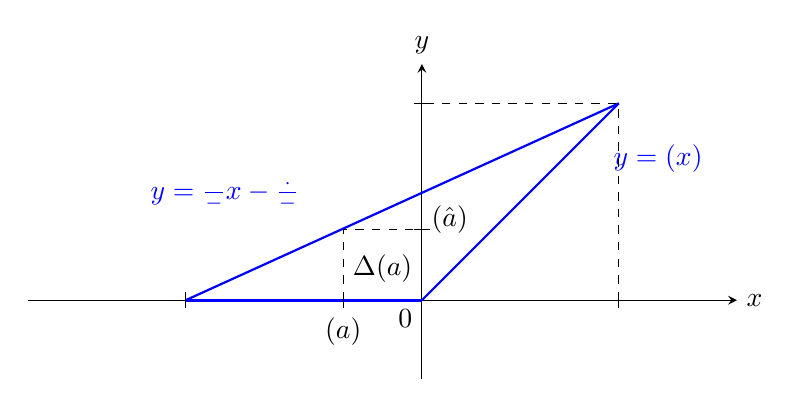
\begin{tikzpicture}[scale=1, >=stealth]
	
	% Draw axes
	\draw[->] (-5,0) -- (4,0) node[right] {$x$};
	\draw[->] (0,-1) -- (0,3) node[above] {$y$};
	
	% Draw ReLU function
	\draw[line width=0.4mm, blue] (-3,0) -- (0,0);
	\draw[thick, blue] (0,0) -- (2.5,2.5) node[below, shift={(0.5,-0.4)}] {$y = \ReLU(x)$};
	\draw[thick, blue] (-3,0) -- (2.5,2.5) node[above, shift={(-5,-1.5)}] {$y = \frac{\UB}{\UB-\LB} x-\frac{\UB\cdot\LB}{\UB-\LB}$};
	
	% Add labels
	\draw[dashed] (2.5,0) -- (2.5,2.5) -- (0,2.5); % Optional grid
	\node[below left] at (0,0) {$0$};
	
	% Add tick marks
	
	\foreach \x in {2.5}
	\draw[shift={(\x,0)}] (0,0.1) -- (0,-0.1) node[below] {$\UB$};
	\foreach \x in {-3}
	\draw[shift={(\x,0)}] (0,0.1) -- (0,-0.1) node[below] {$\LB$};

	\foreach \y in {2.5}
	\draw[shift={(0,\y)}] (0.1,0) -- (-0.1,0) node[left] {$\UB$};
	
	\draw (-1,0.1) -- (-1,-0.1) node[below] {$\sol(a)$};
	\draw[dashed] (-1,0) -- (-1,0.9) -- (0,0.9);
	\draw (-0.1,0.9) -- (0.1,0.9) node[right, shift={(-0.1,0.13)}] {$\sol(\hat{a})$};
	\node at (-0.5,0.4) {$\Delta(a)$};
	
\end{tikzpicture}
	\caption{}
\label{img:Utility}
\end{figure}

\subsection*{An example when FSB is not accurate}

See the figure \ref{img:FSB_example}. When the algorithm considers neurons in the layer of $a,a'$, FSB will think $a$ is important, but Utility will think it is not important (Utility value is 0).

Although this example is extreme, similar situations frequently occur in practice.

\subsection*{Comparison on MNIST}

Here we use the network named MNIST $5\times 100$ and a hard image to compare the effect of FSB and Utility function. 

We fix an intermediate bound data for layers before the third hidden layer, and use different methods based on this bound to compute the upper and lower bounds of neurons in the second and third hidden layer.

The plot shows that when only considering neurons in one layer before the target layer, we are significantly better.


\subsection*{Comparison on CIFAR10}

Here we use the network named CNN-B-adv and a hard image to compare the effect of FSB and Utility function. 

We fix an intermediate bound data for layers before the target layers, and use different methods based on this bound to compute the output layer.

The plot shows that our Utility function is significantly better than FSB, and other methods.

